
\de{ĐỀ THI GIỮA HỌC KỲ II NĂM HỌC 2022-2023}{THPT Marie Curie}

\begin{bt}%[Dự án đề kiểm tra GHKII NH22-23- Dương Phước Sang]%[Marie Curie]%[0T3B2-4]
		\immini{
			Cho hàm số $f(x)=ax^2+bx+c$ có đồ thị $(C)$ như hình vẽ.
			\begin{enumerate}
				\item Từ đồ thị hãy xác định dấu của hệ số $a$ và $\Delta $. 
				\item Tìm tập nghiệm của bất phương trình $f(x)<0$.
			\end{enumerate}}
		{\vspace{-0.5cm}
			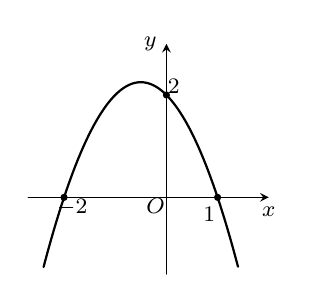
\begin{tikzpicture}[line join=round, line cap=round,>=stealth,font=\footnotesize,scale=0.65]
				\draw[->] (-2.7,0)--(2,0) node[below ] {$x$};
				\draw[->] (0,-1.5)--(0,3) node[left] {$y$};
				\draw (0,0) node [below left=-3pt] {$O$} (1,0) node [below,xshift=-3] {$1$} (-2,0) node [below right=-3pt,xshift=-3] {$-2$} (0,2) node [above right=-3pt] {$2$};
				;
				\fill (1,0) circle (2pt);
				\fill (-2,0) circle (2pt);
				\fill (0,2) circle (2pt);
				\foreach \x in {}
				\draw[thin] (\x,1pt)--(\x,-1pt) node [below] {$\x$};
				\foreach \y in {}
				\draw[thin] (1pt,\y)--(-1pt,\y) node [left] {$\y$};
				\draw[thick,samples=200,domain=-2.4:1.4,smooth,variable=\x] plot (\x,{-1*(\x)^2-1*(\x)+2});
				
		\end{tikzpicture}	}
		\loigiai{
			\begin{enumerate}
				\item Do đồ thị là parabol có bề lõm quay xuống nên $a<0$.\\
				Ngoài ra đồ thị hàm số cắt trục $ Ox $ tại hai điểm phân biệt nên $\Delta >0$.\\
				Như vậy $\heva{&a<0\\&\Delta>0.}$
				\item Dựa vào đồ thị, ta thấy $ f(x)<0 \Leftrightarrow x \in (-\infty;-2) \cup (1;+\infty)$.\\ 
				Vậy bất phương trình $f(x)<0$ có tập nghiệm $S=(-\infty;-2) \cup (1;+\infty)$.
				
			\end{enumerate}
			
		}
	\end{bt}

	\begin{bt}%[Dự án đề kiểm tra GHKII NH22-23- Dương Phước Sang]%[Marie Curie]%[0T7K2-1]
		Tìm tập xác định của hàm số $y=\dfrac{\sqrt{4-x^2}}{x}+\dfrac{2}{\sqrt{x^2-4x+3}}$.
		\loigiai{
			Điều kiện xác định: $ \heva{&4-x^2 \geq 0\\&\quad x \neq 0\\&x^2-4x+3>0} \Leftrightarrow \heva{&-2 \leq x \leq 2\\&\quad x\neq 0\\& \hoac{&x<1\\&x>3}} \Leftrightarrow x\in [-2;1)\setminus \{0\}$.\\
			Vậy $\mathscr{D}=[-2;1) \setminus \{0\} $ là tập xác định của hàm số.
		}
	\end{bt}

	\begin{bt}%[Dự án đề kiểm tra GHKII NH22-23- Dương Phước Sang]%[Marie Curie]%[0T7K2-3]
		Tìm tất cả các giá trị của tham số $m$ để hàm số $f(x)=(3m+1){x^2}-(3m+1)x+m+4$ là tam thức bậc hai âm với mọi $x\in \mathbb{R}$.
		\loigiai{
			\textbf{Trường hợp 1:} $3m+1=0 \Leftrightarrow m=-\dfrac{1}{3} $ thì $ f(x)=\dfrac{11}{3}>0 $ với mọi $x\in \mathbb{R}$.\\
			Như thế, $ m= -\dfrac{1}{3}$ không thỏa mãn yêu cầu của bài toán.\\
			\textbf{Trường hợp 2:} $ m \neq -\dfrac{1}{3} $ thì yêu cầu bài toán xảy ra khi và chỉ khi 
			$$\heva{&a<0\\&\Delta <0} 
			\Leftrightarrow
			\heva{&3m+1<0\\&(3m+1)^2-4(3m+1)(m+4)<0}
			\Leftrightarrow \heva{&m<-\dfrac{1}{3}\\&\hoac{&m<-15\\&m>-\dfrac{1}{3}}}\Leftrightarrow m<-15.$$
		}
	\end{bt}

	\begin{bt}%[Dự án đề kiểm tra GHKII NH22-23- Dương Phước Sang]%[Marie Curie]%[0T7B3-2]
		Giải các phương trình sau
		\begin{listEX}[2]
			\item $2x+\sqrt{x^2-2x+6}=1$.
			\item $\sqrt{3x^2-6x-5}=\sqrt{x^2-9}$.
		\end{listEX}
		\loigiai{
			\begin{enumerate}
				\item $2x+\sqrt{x^2-2x+6}=1 \Leftrightarrow \sqrt{x^2-2x+6}=1-2x $.\\
				Bình phương hai vế của phương trình, ta được $ 3x^2-2x-5=0 \Leftrightarrow \hoac{&x=-1\\&x=\dfrac{5}{3}.}$\\
				Thử lại, ta được $ S=\left\{-1\right\}$ là tập nghiệm của phương trình đã cho.
				\item $\sqrt{3x^2-6x-5}=\sqrt{x^2-9}$.\\
				Bình phương hai vế của phương trình, ta được $ 2x^2-6x+4=0 \Leftrightarrow \hoac{&x=1\\&x=2.}$\\
				Thử lại, ta thấy không có số $x$ nào thỏa mãn phương trình, do đó phương trình vô nghiệm.
			\end{enumerate}
		}
	\end{bt}

	\begin{bt}%[Dự án đề kiểm tra GHKII NH22-23- Dương Phước Sang]%[Marie Curie]%[0T9B2-2]
		Trong mặt phẳng tọa độ $Oxy$, cho tam giác $ABC$ với $A(-4;3)$, $B(-1;2)$ và $C(-3;6)$.
		\begin{enumerate}
			\item	Viết phương trình tổng quát đường thẳng $d_1$ là đường trung bình của tam giác $ABC$ song song với cạnh $BC$.
			\item Viết phương trình tham số của đường thẳng $d_2$ qua điểm $C$ và vuông góc đường cao $CH$.
		\end{enumerate}
		\loigiai{
			\begin{enumerate}
				\item Gọi $ M$, $N $ lần lượt là trung điểm $ AB$, $AC $.\\
				Suy ra $ M\left(-\dfrac{5}{2};\dfrac{5}{2}\right) $ và $ N\left(-\dfrac{7}{2};\dfrac{9}{2}\right) $
				nên $ \overrightarrow{MN}=(-1;2) $ là một véc-tơ chỉ phương của $d_1$.\\
				$ d_1 $ đi qua $ M $ và nhận $ (2;1) $ là véc-tơ pháp tuyến nên có phương trình $ 2x+y+\dfrac{5}{2}=0 $.
				\item $ d_2 $ qua $ C $ và song song $ AB $ nên nhận $ \overrightarrow{AB}=(3;-1) $ là véc-tơ chỉ phương.\\
				Suy ra $ d_2 \colon \heva{&x=-3+3t\\&y=6-t.}$
			\end{enumerate}	
			
		}
	\end{bt}

	\begin{bt}%[Dự án đề kiểm tra GHKII NH22-23- Dương Phước Sang]%[Marie Curie]%[0T9K2-6]
		Cho đường thẳng đường thẳng $\Delta\colon 2x-y+10=0$ và điểm $M(1 ;-3)$. Tìm tọa độ điểm $N$ thuộc đường thẳng $\Delta $ sao cho độ dài đoạn $MN$ là nhỏ nhất.
		\loigiai{
			Ta có $2x-y+10=0 \Leftrightarrow y=2x+10 \Leftrightarrow \heva{&x=t\\&y=2t+10.}$\\
			Vì $ N \in \Delta$ nên $ N(t; 2t+10) $ và $ \overrightarrow{MN}=(t-1; 2t+13) $.\\
			Suy ra $ MN=\sqrt{5t^2+50t+170} $.\\
			Do $f(t)=5t^2+50t+170$ là hàm số bậc hai theo $t$, đạt giá trị nhỏ nhất tại $t=-5$.\\
			Từ đó với $N(-5; 0)$ thì $N \in \Delta$ và $MN$ nhỏ nhất.
		}
	\end{bt}
